\documentclass{article}

\usepackage[utf8]{inputenc}

\usepackage{amsmath, bm}
\usepackage{graphicx}
\usepackage{amssymb}
\usepackage{float}
\usepackage{caption}
\usepackage{subcaption}
% set font size to 11pt
% set margin
\usepackage[margin=0.5in]{geometry}

\setlength{\parskip}{\baselineskip}%
\setlength{\parindent}{0pt}%

\begin{document}

% insert pdf cover page here

\title{Lab report: 3A3 Supersonic Nozzle}
\author{lwp26}
\date{October 2023}
\maketitle

\begin{abstract}
    \centering
    % write a brief summary of the experiment and the results
    Uhm this is the abstract which will be written at the end!
\end{abstract}

\section{Introduction}

\subsection{Purpose}
% explaining the significance of supersonic nozzles to wind tunnels and other applications.
% The converging-diverging nozzle is a device that can accelerate a fluid to supersonic speeds, and is used in both aircraft and wind tunnels.
The converging-diverging nozzle is a device that can accelerate a fluid to supersonic speeds, and is used in many engineering applications, such as the design of supersonic wind tunnels, supersonic aircraft and rocket engines.
Supersonic nozzles are essential components in wind tunnels designed to simulate high-speed conditions that objects experience in flight.
By accelerating airflow to supersonic speeds, these nozzles enable researchers to recreate the aerodynamic forces and flow patterns that occur at high speeds.
This is also done at a smaller scale through dimensional analysis which significantly reduces the cost of testing.

% explain the purpose of the experiment

\subsection{Objectives}
% list the objectives of the experiment

\begin{itemize}
    \item To study the static pressure distribution in a converging-diverging nozzle for 4 different pressure ratios across the nozzle.
    \item To appreciate the validity and limitations of one-dimensional, adiabatic, inviscid theory for calculating mass flow rate from the pressure drop across an oriface plate.
    \item 
\end{itemize}

\section{Theory}
% Introduce the essential relationships necessary to explain your results in the later section. Refer to these
% equations in the later sections. (You need not derive these relationships but you should explain in words why
% they are needed and reference their source).

\subsection{Mass flow rate though oriface plate}

The following assumptions are made to derive a relationship for the mass flow rate through an orifice plate.
\begin{itemize}
    \item The flow into the orifice is inviscid,
    \item The flow is slow enough to be treated as incompressible with density equal to that in the atmosphere upstream of the orifice (where the velocity is negligible),
    \item The velocity is uniform across the plane of the orifice,
    \item The pressure difference between the orifice plane and the upstream atmosphere is that measured on the water manometer
\end{itemize} 

With both the invicid and incompressible assumptions, the ideal flow rate through the orifice can be calculated using the pressure difference between the orifice plane and the upstream atmosphere is that measured on the
water manometer. By applying the Bernoulli equation from the upstream atmosphere (1) to the orifice plane (2),

\begin{equation}
    p_1 = p_2 + \frac{1}{2} \rho_a v_2^2
\end{equation}

Where $A$ and $v_2$ are the cross-sectional area, and velocity at the orifice. The pressure in the centre of the oriface is taken to be equal to the value measured at the wall, due to the assumption that the velocity is uniform across the oriface plane.
The theoretical mass flow rate through the orifice is then given by the following equation.
\begin{equation}
    \dot{m}_{ideal} = \rho_a A v_2 = \rho_a \left( \frac{\pi D^2}{4}\right) \sqrt{\frac{2(p_1-p_2)}{\rho_a}} \;\;\;\;\;\; \text{where} \;\;\;\;\;\ p_2 - p_1 = \rho_w g \Delta h
\end{equation}
Where $\rho_a$ is the density of air and $\rho_w$ is the density of water used for the manometer.

However, the actual flow rate through the orifice differs from the theoretical value as our assumptions are not valid.
The first assumption is not valid as there is significant viscous dissipation before the orifice. However, these losses are accounted for by a discharge coefficient $C_d$, which is defined as the ratio of actual discharge to the ideal discharge.
The value of $C_d$ is constant at the high Reynolds numbers considered in this report.
To analyse the validity of the second assumption, consider the case of maximum flow, when the nozzle is choked upstream of the orifice, then its non-dimensional mass flow rate is given by the following equation.
\begin{equation}
    \frac{\dot{m}\sqrt{c_pT_0}}{p_0A^*} = 1.281
\end{equation}
From this, the non-dimensional mass flow rate at the orifice can be calculated using the area ratio of the orifice to the nozzle throat.
The area of the throat is approximately $24\text{mm}^2$, and so the non-dimensional mass flow rate at the orifice is $0.1282$.
At this point, the corresponding density ratio $\rho/\rho_0 = 0.9997 \approx 1$. This means that the density change is negligible and can be ignored.

The third assumption that the velocity is uniform is also poor, and is accounted for by the discharge coefficient $C_d$.
This difference is characterised by the discharge coefficient $C_d$ which is defined as the ratio of the actual flow rate to the theoretical flow rate.
\begin{equation}
    \dot{m}_{actual} = C_d \dot{m}_{ideal}
\end{equation}

The discharge coefficient of the orifice is effectively constant over the range of high reynolds numbers considered in this experiment.
This was shown by Graham and Webster \cite{Graham_K_Webster:2019} in figure \ref{fig:const_Cd_Re}.

\subsection{Pressure tappings}

The static pressure at a specific pressure tapping along the nozzle is given by the following equation.
\begin{equation}
    p = p_0 - \rho_{Hg} g \Delta h
\end{equation}
Where $\rho_{Hg}$ is the density of mercury and $\Delta h$ is the height difference of mercury between the specific pressure tapping and atmospheric tapping.
The ratio of this with the stagnation pressure (atmospheric pressure) is the static to stagnation pressure ratio which is plotted below in figure \ref{fig:figure4}.

\subsection{Shlieren visualisation technique}

Mazumdar et al. \cite{Mazumdar_Amrita:2013} describes the Shlieren visualisation technique as a method of visualising the density gradient of a fluid.

\begin{figure}[H]
    \centering
    \begin{subfigure}[t]{0.48\textwidth}
        \centering
        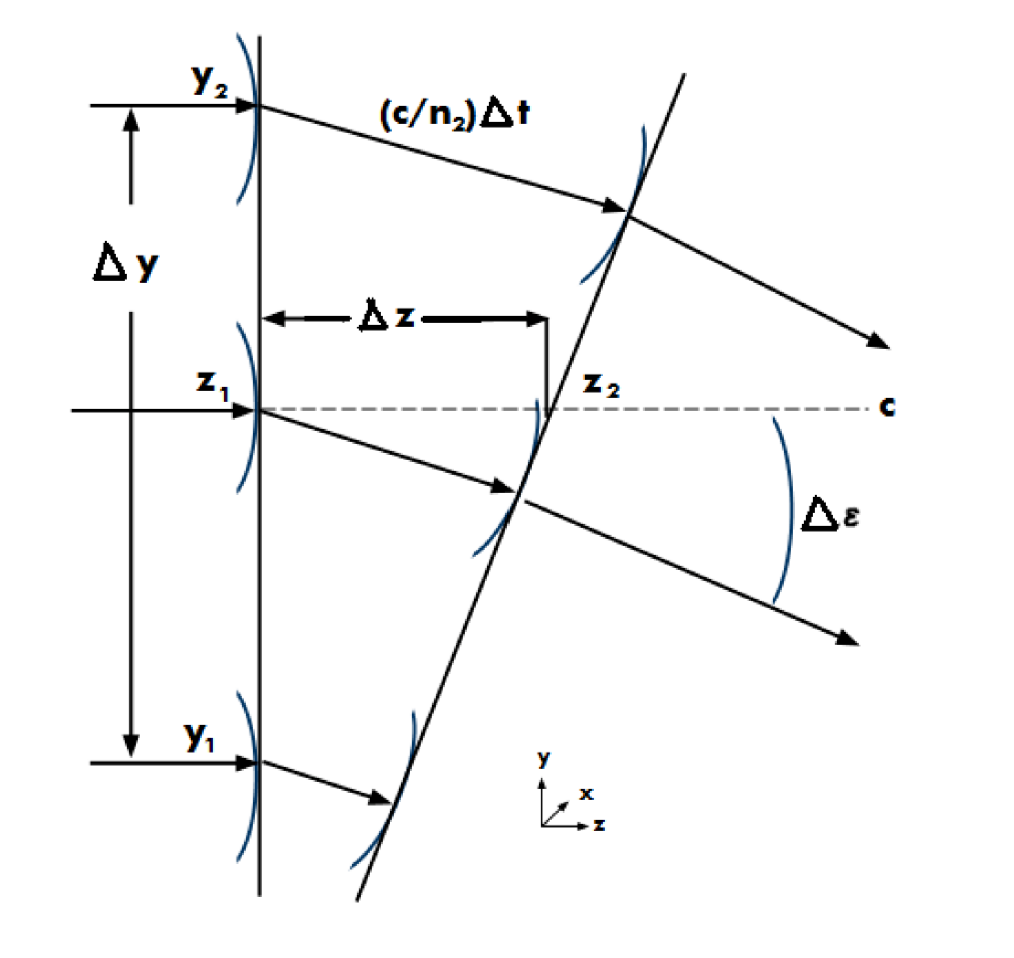
\includegraphics[width=1\textwidth]{Mazumdar_Amrita_shlierien_refraction.png}
        \caption{heading}
        \label{fig:mirror_setup}
    \end{subfigure}
    ~
    \begin{subfigure}[t]{0.48\textwidth}
        \centering
        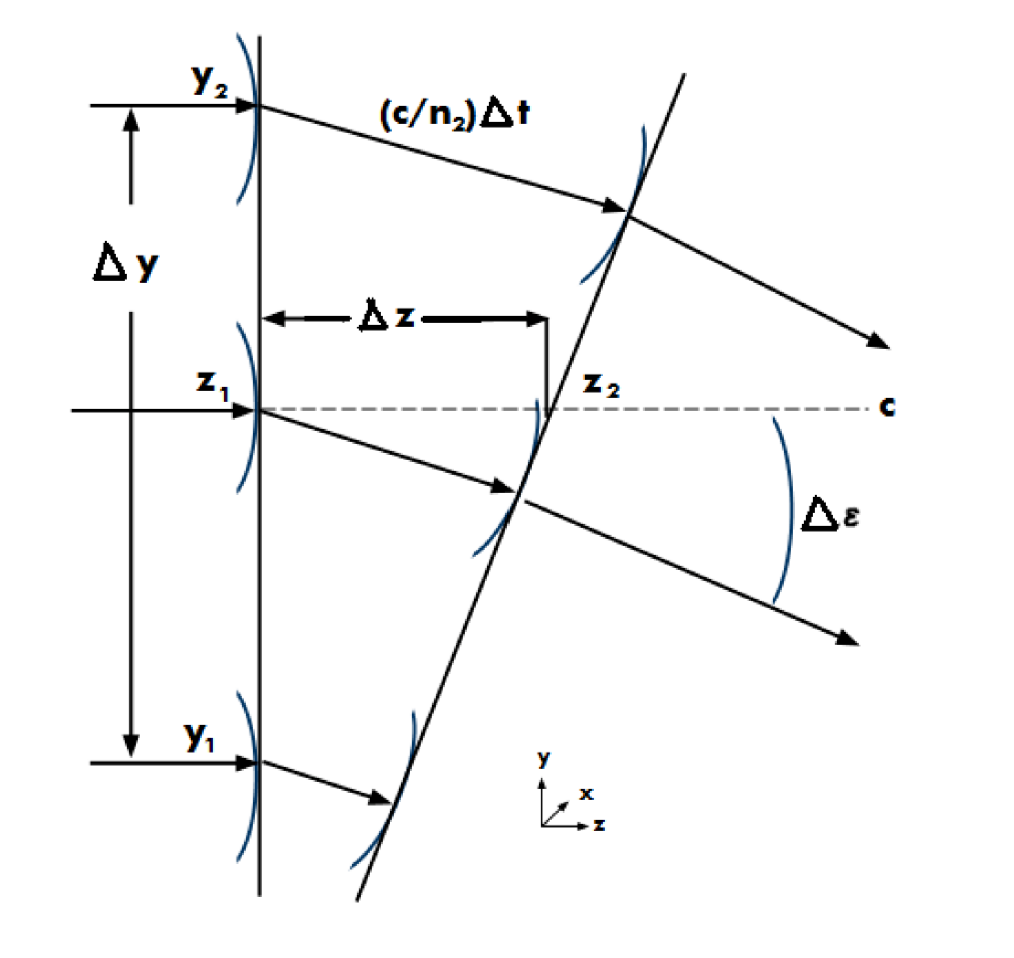
\includegraphics[width=1\textwidth]{Mazumdar_Amrita_shlierien_refraction.png}
        \caption{Top down view of light ray deflection in mediums of different refractive indices \cite{Mazumdar_Amrita:2013}.}
        \label{fig:refraction_diagram}
    \end{subfigure}
    \caption{Shlieren visualisation technique \cite{Mazumdar_Amrita:2013}.}
\end{figure}

\begin{equation}
    \frac{d\theta}{dx} = \frac{1}{n} \frac{dn}{dx}
\end{equation}

Equation 1 indicates it is not the refractive index n causing ray deflection, but the gradient of
this refractive index. Additionally, Eqns. 1 and 2 show light ray deflections bend towards regions of higher
refractive index


\section{Method}

\subsection{Part 1}

\subsubsection{Apparatus}

\begin{figure}[H]
    \centering
    \begin{subfigure}{0.8\textwidth}
        \centering
        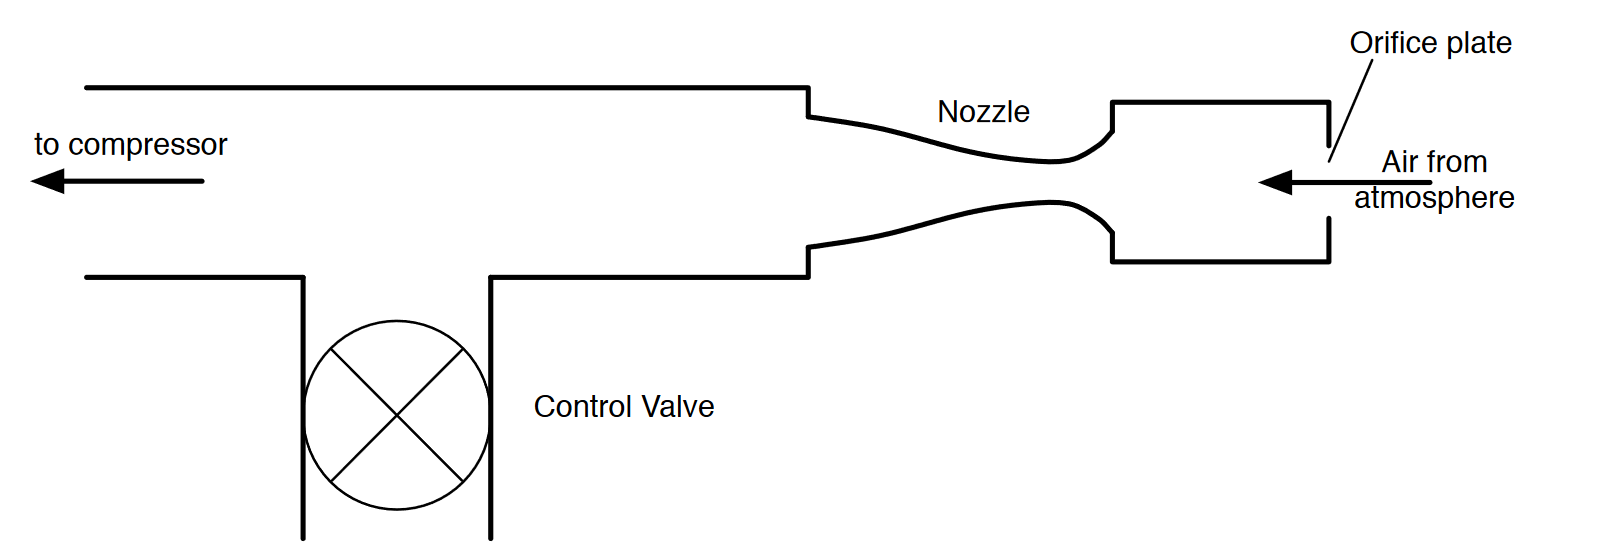
\includegraphics[width=0.6\textwidth]{flow_layout.png}
        \caption{Flow path diagram}
        \label{fig:flow_layout}
    \end{subfigure}
    ~
    \begin{subfigure}{0.8\textwidth}
        \centering
        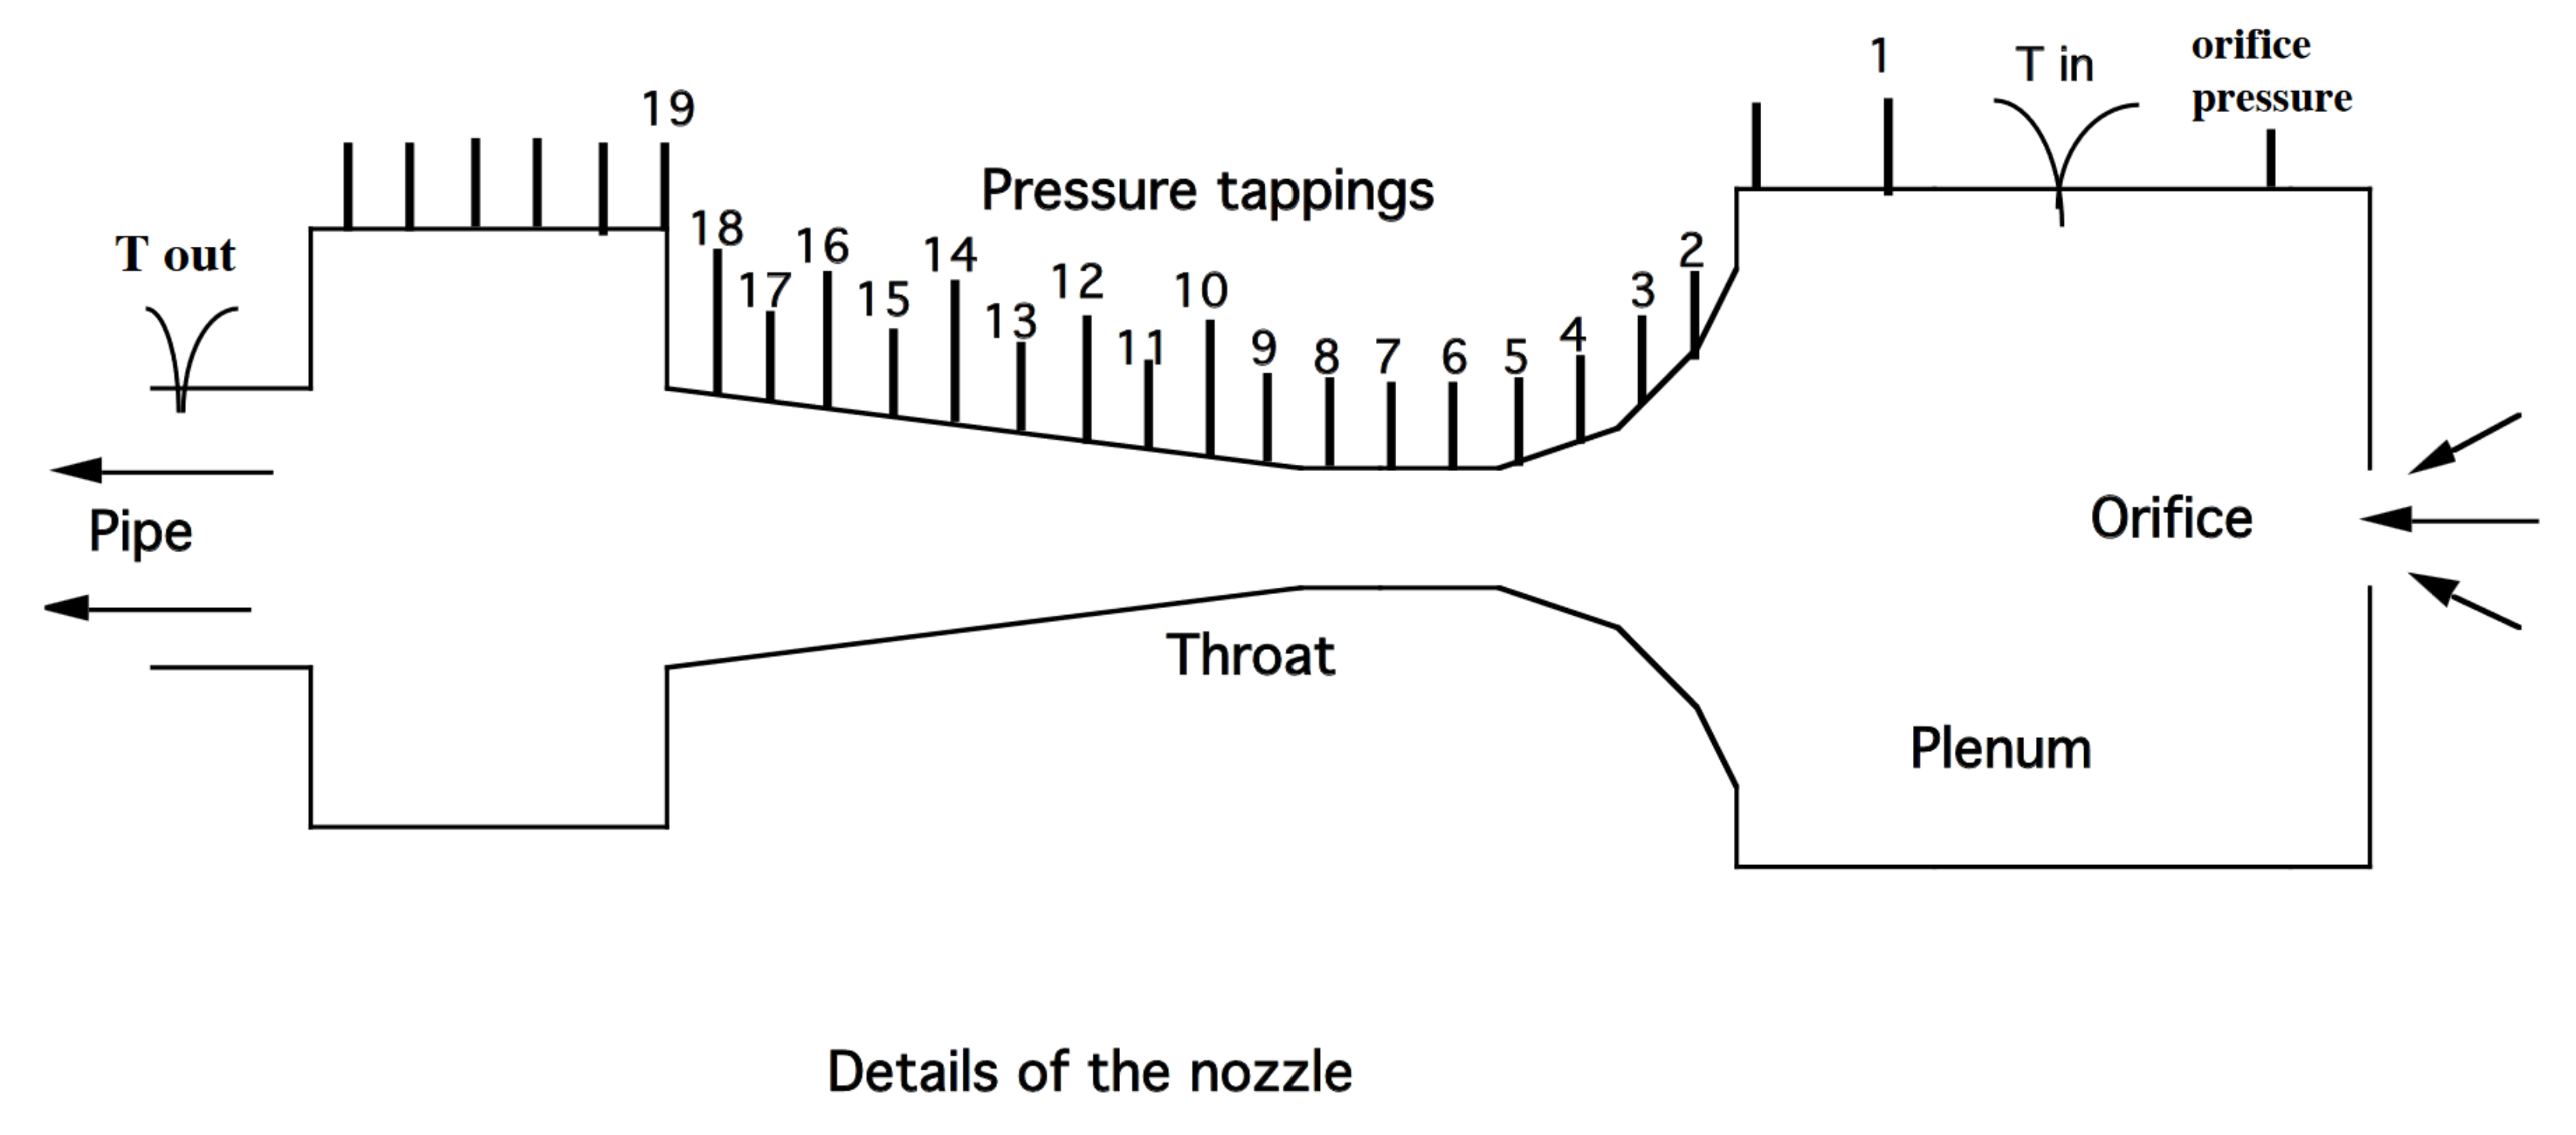
\includegraphics[width=0.6\textwidth]{../Supersonic_Nozzle/small_nozzle_layout.png}
        \caption{Nozzle layout diagram}
        \label{fig:nozzle_layout}
    \end{subfigure}
    \caption{Experiment apparatus \cite{lab_manual}.}
\end{figure}

The apparatus used in this experiment is shown in figure \ref{fig:flow_layout}.
A control valve is used to control the pressure of the air downstream of the nozzle. By closing the valve, the pressure downstream of the nozzle decreases, and so pressure ratio across the nozzle increases.
The pressure at each tapping along the nozzle is measured using a series of 19 vertical mercury manometers.
The pressure difference accross the oriface is a smaller pressure drop and so is measured using a vertical water manometer.

\subsubsection{Procedure}

A preliminary experiment was conducted to determine the pressure ratio at which the nozzle is choked.
This was done by increasing the pressure ratio across the nozzle until there was no change in the oriface plate manometer readings.
This approximate height difference of the manometer at the choking point was then recorded.

Then we started the main experiment by setting the height difference of the manometer to $70\%$ of that of the choking point.

\subsection{Part 2}

\subsubsection{Procedure}

\subsubsection{Apparatus}

\section{Results}


\begin{figure}[H]
    \centering
    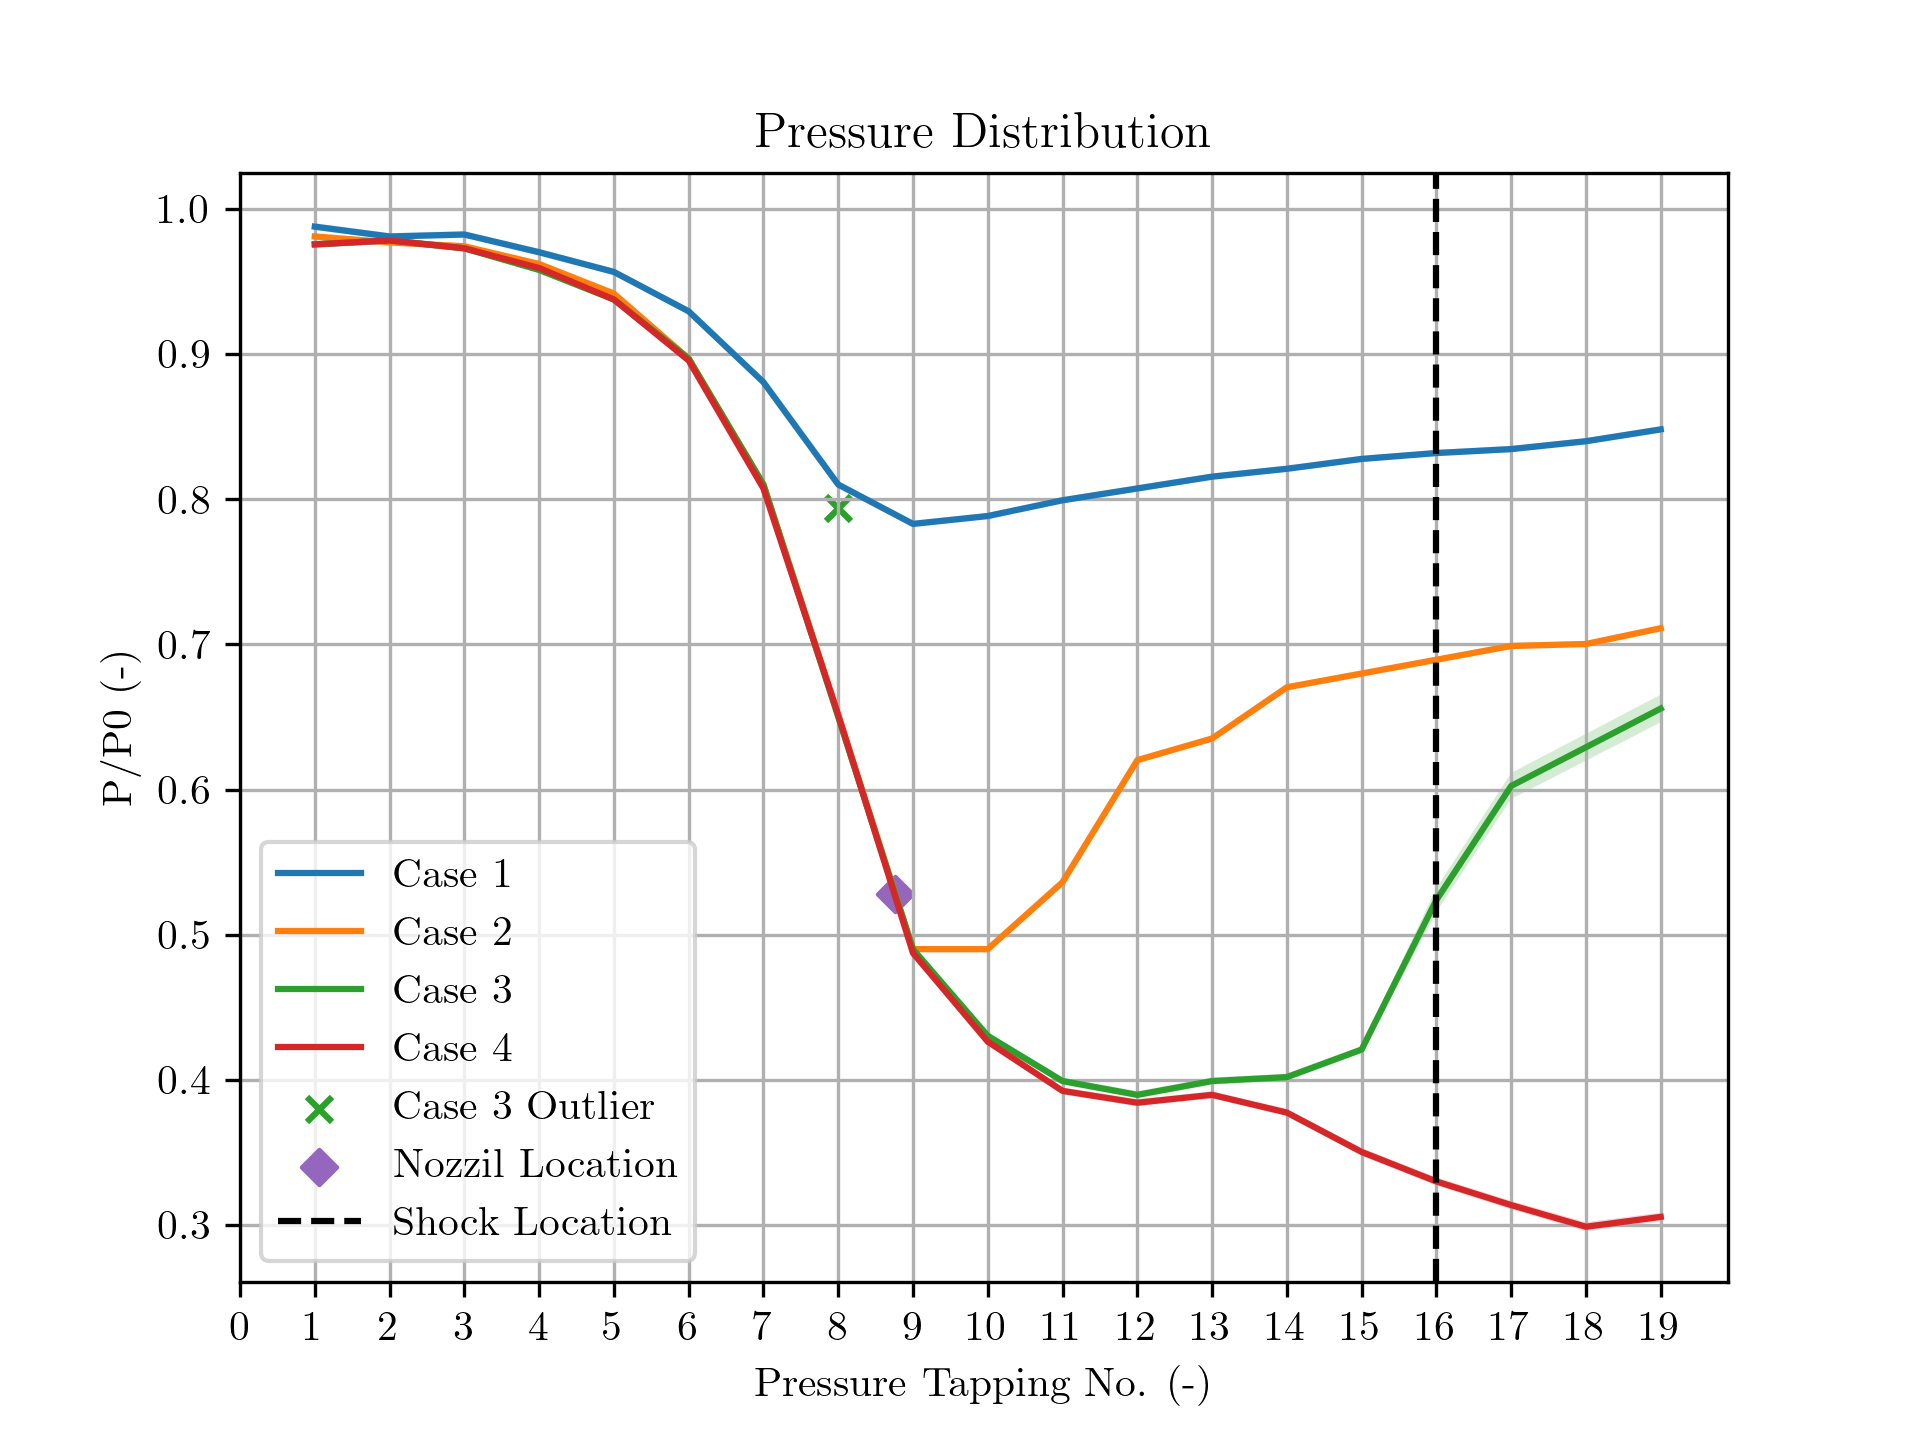
\includegraphics[width=0.8\textwidth]{../Supersonic_Nozzle/pressure_ratio_distribution_corrected.png}
    \caption{Static pressure ratio distribution along the nozzle.}
    \label{fig:figure4}
\end{figure}

\begin{figure}[H]
    \centering
    \begin{subfigure}[t]{0.48\textwidth}
        \centering
        \includegraphics[width=1\textwidth]{../Supersonic_Nozzle/shadowgraph_annotations/slide1.PNG}
        \caption{Shock wave in working section before sensors}

        \label{fig:figure6}
    \end{subfigure}
    ~
    \begin{subfigure}[t]{0.48\textwidth}
        \centering
        \includegraphics[width=1\textwidth]{../Supersonic_Nozzle/shadowgraph_annotations/slide2.PNG}
        \caption{Working state and bow shock of pitot probe}
        \label{fig:figure7}
    \end{subfigure}
    \caption{Shadowgraph images of the supersonic wind tunnel}
\end{figure}

\section{Discussion}

\section{Conclusion}
% Comment on the validity of one-dimensional theory in nozzle flows. When can it be expected to provide what quality of predictions?
% What are the effects of viscosity in both experiments? Which experiment is more severely affected and why?

\newpage

\section{Appendix}


The following equations are used to correct for the drop in stagnation pressure accross the shock wave in Case 3.

\begin{equation}
    \frac{p_{0s}}{p_0} = \left( \frac{\frac{\gamma+1}{2}M^2}{1 + \frac{\gamma-1}{2}M^2}\right) ^ \frac{\gamma}{\gamma-1} \left( \frac{2\gamma}{\gamma+1} M^2 - \frac{\gamma-1}{\gamma+1}\right) ^ \frac{1}{1 - \gamma}
\end{equation}

\begin{equation}
    u\left( \frac{p_{0s}}{p_0} \right) = u(M) \frac{d}{dM}\left( \frac{p_{0s}}{p_0} \right)
\end{equation}

\begin{equation}
    \begin{aligned}[b]
    & \frac{d}{dM}\left( \frac{p_{0s}}{p_0} \right) = - \frac{4 M \gamma \left(\frac{M^{2} \left(\frac{\gamma}{2} + \frac{1}{2}\right)}{M^{2} \left(\frac{\gamma}{2} - \frac{1}{2}\right) + 1}\right)^{\frac{\gamma}{\gamma - 1}} \left(\frac{2 M^{2} \gamma}{\gamma + 1} - \frac{\gamma - 1}{\gamma + 1}\right)^{- \frac{1}{\gamma - 1}}}{\left(\gamma - 1\right) \left(\gamma + 1\right) \left(\frac{2 M^{2} \gamma}{\gamma + 1} - \frac{\gamma - 1}{\gamma + 1}\right)} \\
    & + \frac{\gamma \left(\frac{M^{2} \left(\frac{\gamma}{2} + \frac{1}{2}\right)}{M^{2} \left(\frac{\gamma}{2} - \frac{1}{2}\right) + 1}\right)^{\frac{\gamma}{\gamma - 1}} \left(M^{2} \left(\frac{\gamma}{2} - \frac{1}{2}\right) + 1\right) \left(\frac{2 M^{2} \gamma}{\gamma + 1} - \frac{\gamma - 1}{\gamma + 1}\right)^{- \frac{1}{\gamma - 1}} \left(- \frac{2 M^{3} \left(\frac{\gamma}{2} - \frac{1}{2}\right) \left(\frac{\gamma}{2} + \frac{1}{2}\right)}{\left(M^{2} \left(\frac{\gamma}{2} - \frac{1}{2}\right) + 1\right)^{2}} + \frac{2 M \left(\frac{\gamma}{2} + \frac{1}{2}\right)}{M^{2} \left(\frac{\gamma}{2} - \frac{1}{2}\right) + 1}\right)}{M^{2} \left(\frac{\gamma}{2} + \frac{1}{2}\right) \left(\gamma - 1\right)}
    \end{aligned}
    \label{eqn:dp0sr_dm}
\end{equation}
\footnotetext{Equation \ref{eqn:dp0sr_dm} was generated using SymPy}

\begin{figure}[H]
    \centering
    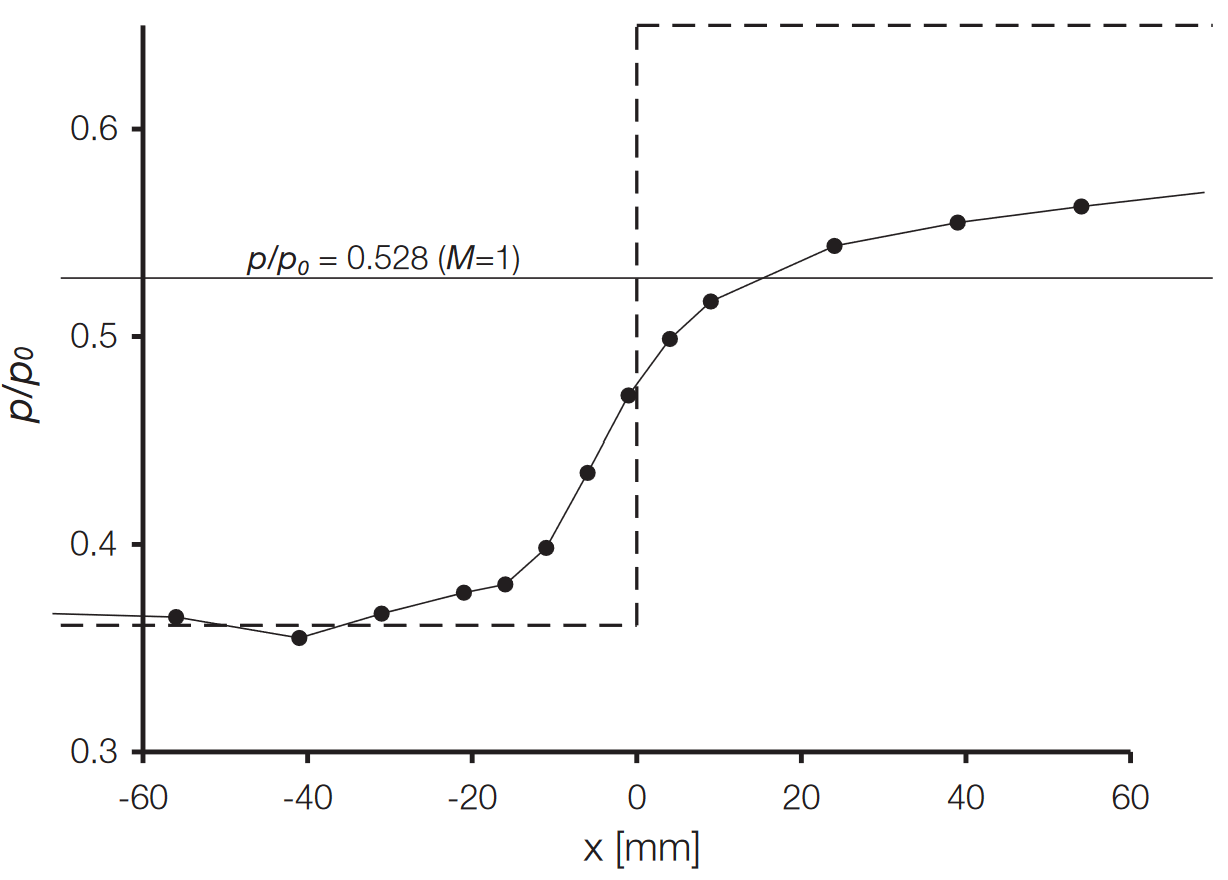
\includegraphics[width=0.6\textwidth]{SBLI_pressure_smearing.png}
    \caption{Static wall pressure distribution at the shock boundary layer interaction \cite{babinsky_delery:2011}.}
    \label{fig:SBLI_pressure_smearing}
\end{figure}

\begin{figure}[H]
    \centering
    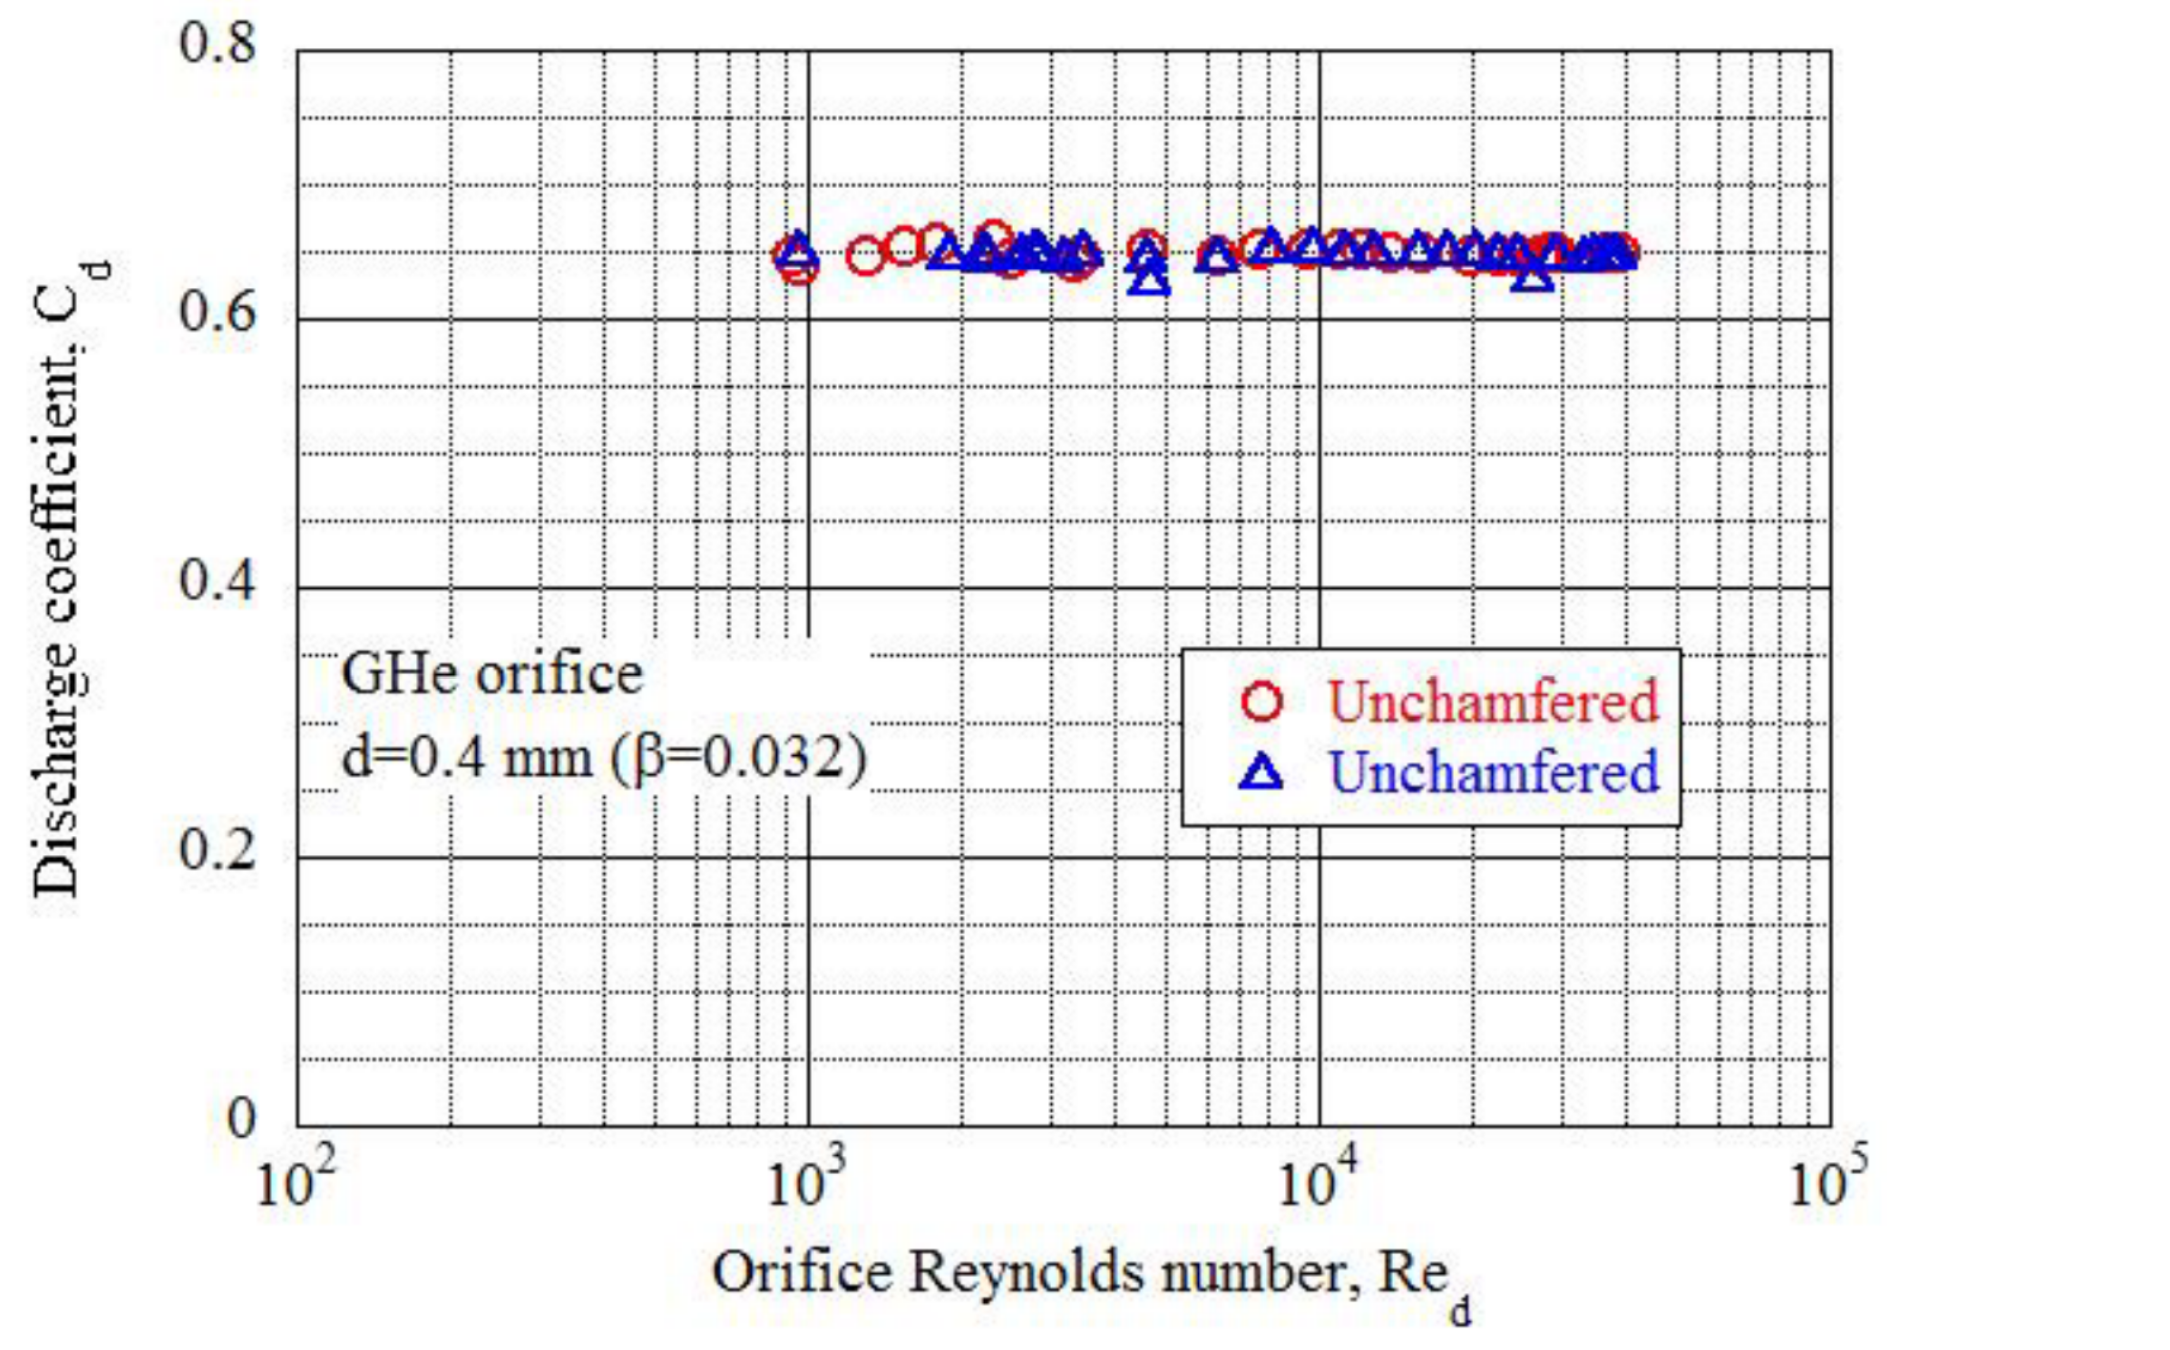
\includegraphics[width=0.6\textwidth]{Graham_K_Webster_const_Cd_Re.png}
    \caption{Constant discharge coefficient for high Reynolds numbers \cite{Graham_K_Webster:2019}.}
    \label{fig:const_Cd_Re}
\end{figure}

\bibliographystyle{plain} % We choose the "plain" reference style
\bibliography{refs} % Entries are in the refs.bib file

\end{document}